\begin{refsection}

\section{Introduction}
\label{sec:introduction}

\subsection{Motivation for Fuel Performance Modelling}

Nuclear fuel rods operate under demanding conditions: high power densities which drive temperatures well above 1000\,\textdegree C, while the surrounding cladding must remain structurally sound under coolant pressure, internal fission gas accumulation, and irradiation damage.  A quantitative model of the evolving thermal and mechanical state of the fuel rod is therefore necessary for:

\begin{itemize}
\item \textbf{Safety margins}: verifying that fuel and cladding temperatures, stresses, and strains remain within regulatory and design limits during steady-state operation and transient events;
\item \textbf{Design optimisation}: exploring the effect of pellet geometry (e.g.\ annular pellets), gap width, cladding thickness, and fill-gas composition on performance without expensive in-pile experiments;
\item \textbf{Material qualification}: comparing candidate fuel and cladding materials (oxide, metallic, carbide fuels; austenitic, ferritic and refractory claddings) through a common simulation framework;
\item \textbf{Irradiation programme planning}: predicting end-of-life condition to support post-irradiation examination (PIE) campaigns.
\end{itemize}

Historically, the original FRED fuel performance code was a Fortran program written specifically to model the properties of Mixed Oxide (MOX) fuels for fast spectrum systems. However, growing interest in alternative fuel forms, such as metallic fuel and uranium nitride, has introduced a need for fuel-system-specific residual formulations capable of capturing base irradiation behaviour and fuel-cladding-coolant interactions unique to each fuel system. This has motivated the development of a new version of FRED, designed with a focus on developer experience and tight integration within experimental-modelling pipelines. To avoid duplication of code, a common physics solver library is employed, particularly in the implementation of the stress-strain and thermal balance residual equations.

The FRED platform adopts a modular, object-oriented architecture: the core equations governing heat conduction and stress-strain are implemented once in the \emph{platform layer}, while reactor-system-specific material correlations and additional physics (fission gas release, swelling, etc.) are implemented as \emph{application layers} built on top~\cite{hindmarsh2005}.

\subsection{Overview of FRED 2.0}

FRED 2.0 is a C\texttt{++} fuel performance platform with a Python scripting interface (via \texttt{pybind11}) and the SUNDIALS IDA solver for time integration of implicit differential-algebraic equation (DAE) systems \cite{hindmarsh2005}.  Three applications are currently available:

\begin{description}
\item[\textbf{FRED-ROD}] Pure thermo-mechanical solver with no irradiation model.  Suitable for out-of-pile thermal tests, gap-closure studies, and material property testing.  Any user-defined fuel and cladding material can be plugged in through the python API abstract material interfaces.

\item[\textbf{FRED-OX}] Mixed oxide (MOX/UO$_2$) fuel in a sodium-cooled environment.  Extends FRED-ROD with burnup tracking, fission gas generation and release (Waltar-Reynolds model~\cite{waltar1981}), fuel swelling (MATPRO~\cite{hagrman1981}), and a fission-gas-corrected gap conductance model.

\item[\textbf{FRED-M-Na}] Metallic fuel (U-Pu-Zr) in sodium.  Extends the platform with irradiation phenomena specific to metallic fuel: fuel swelling from solid fission products, zirconium redistribution, sodium infiltration, and an empirical fission gas release model \cite{karahan2009}.
\end{description}

\subsection{Geometry and Coordinate System}

The fuel rod is modelled as a cylinder with axial symmetry.  The computational domain is discretised in the radial direction into $n_f$ fuel rings and $n_c$ cladding rings, and in the axial direction into $n_z$ layers, as illustrated in Figure~\ref{fig:rz_discretization}.  All equations are solved independently per axial layer (plane-strain assumption) and are coupled through the shared gas inventory and pressure.

\begin{figure}[H]
  \centering
  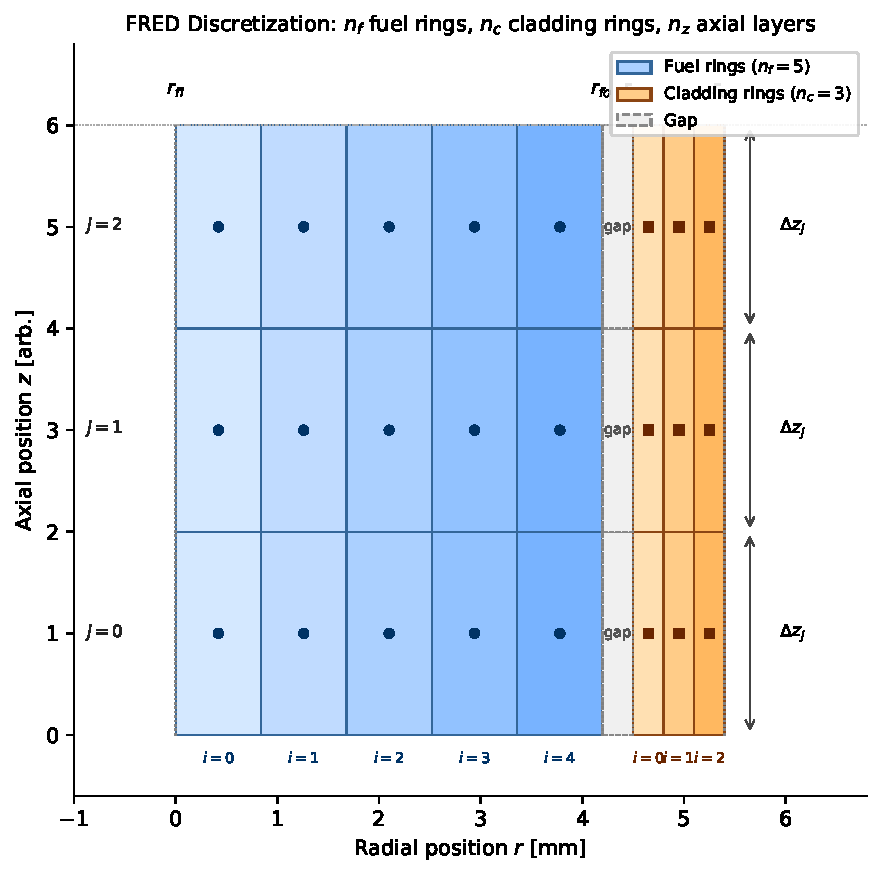
\includegraphics[width=0.85\textwidth]{images/rz_discretization.pdf}
  \caption{Schematic of the FRED radial-axial discretization.  The fuel pellet is divided into $n_f$ concentric rings (blue) and the cladding into $n_c$ rings (orange), separated by the fuel-cladding gap.  Each axial layer~$j$ has height~$\Delta z_j$.  Filled symbols denote the finite-volume node locations.}
  \label{fig:rz_discretization}
\end{figure}

\subsection{Governing Variables}

Table~\ref{tab:variables} lists the primary unknowns tracked at each axial layer and their governing equations.

\begin{table}[H]
  \centering
  \caption{Primary unknowns per axial layer in FRED.}
  \label{tab:variables}
  \begin{tabular}{llll}
    \toprule
    Symbol & Description & Units & Equation type \\
    \midrule
    $T_i$     & Temperature at radial node $i$ & K   & ODE \\
    $\sigma_r$, $\sigma_\theta$, $\sigma_z$ & Stress components & MPa & AE \\
    $\varepsilon_r$, $\varepsilon_\theta$, $\varepsilon_z$ & Strain components & - & AE \\
    $\delta$  & Gap width            & m   & AE \\
    $p_{fc}$  & Contact pressure     & MPa & AE \\
    $h_{gap}$ & Gap conductance      & W/(m$^2$\,K) & AE \\
    $p_{gas}$ & Internal gas pressure & MPa & AE  \\
    \bottomrule
  \end{tabular}
\end{table}

\printbibliography[heading=subbibliography,title={References}]
\end{refsection}
